\definecolor{ctblock}{RGB}{33,102,172}
\definecolor{ctcall}{RGB}{230,145,56}
\definecolor{ctstate}{RGB}{77,146,33}
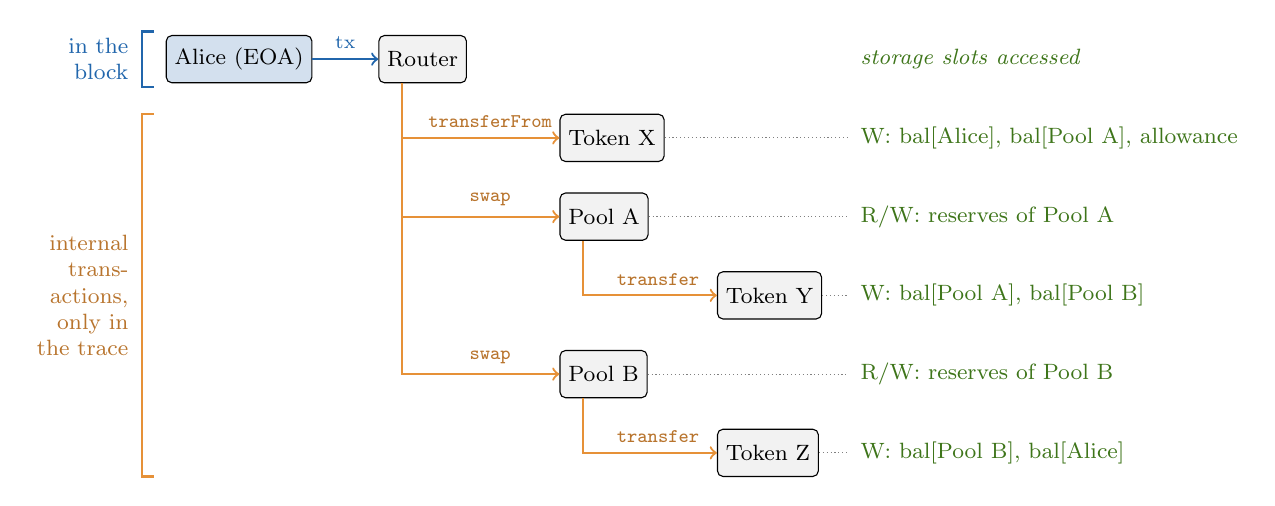
\begin{tikzpicture}[x=1cm,y=1cm,font=\footnotesize,
	acc/.style={draw,rounded corners=2pt,minimum height=0.6cm,inner sep=3pt,anchor=west},
	eoa/.style={acc,fill=ctblock!20},
	ctr/.style={acc,fill=gray!10},
	slots/.style={anchor=west,text=ctstate!80!black},
	call/.style={->,thick,ctcall},
	lbl/.style={font=\scriptsize\ttfamily,text=ctcall!80!black,above,pos=0.78}]
	% Transaction recorded in the block
	\node[eoa] (alice) at (0,0) {Alice (EOA)};
	\node[ctr] (router) at (2.7,0) {Router};
	\draw[->,thick,ctblock] (alice) -- node[above,font=\scriptsize,text=ctblock] {tx} (router);
	% Internal transactions
	\node[ctr] (tx) at (5.0,-1.0) {Token X};
	\node[ctr] (pa) at (5.0,-2.0) {Pool A};
	\node[ctr] (ty) at (7.0,-3.0) {Token Y};
	\node[ctr] (pb) at (5.0,-4.0) {Pool B};
	\node[ctr] (tz) at (7.0,-5.0) {Token Z};
	\coordinate (rs) at ([xshift=0.3cm]router.south west);
	\coordinate (as) at ([xshift=0.3cm]pa.south west);
	\coordinate (bs) at ([xshift=0.3cm]pb.south west);
	\draw[call] (rs) |- node[lbl] {transferFrom} (tx.west);
	\draw[call] (rs) |- node[lbl] {swap} (pa.west);
	\draw[call] (rs) |- node[lbl] {swap} (pb.west);
	\draw[call] (as) |- node[lbl] {transfer} (ty.west);
	\draw[call] (bs) |- node[lbl] {transfer} (tz.west);
	% Storage slots read and written
	\node[anchor=west,text=ctstate!80!black,font=\footnotesize\itshape] at (8.7,0) {storage slots accessed};
	\node[slots] at (8.7,-1.0) {W: bal[Alice], bal[Pool A], allowance};
	\node[slots] at (8.7,-2.0) {R/W: reserves of Pool A};
	\node[slots] at (8.7,-3.0) {W: bal[Pool A], bal[Pool B]};
	\node[slots] at (8.7,-4.0) {R/W: reserves of Pool B};
	\node[slots] at (8.7,-5.0) {W: bal[Pool B], bal[Alice]};
	\foreach \n/\y in {tx/-1,pa/-2,pb/-4} \draw[densely dotted,gray] (\n.east) -- (8.65,\y);
	\foreach \n/\y in {ty/-3,tz/-5} \draw[densely dotted,gray] (\n.east) -- (8.65,\y);
	% Brackets on the left
	\draw[ctblock,thick] (-0.15,0.35) -- (-0.3,0.35) -- (-0.3,-0.35) -- (-0.15,-0.35);
	\node[anchor=east,align=right,text=ctblock] at (-0.35,0) {in the\\block};
	\draw[ctcall,thick] (-0.15,-0.7) -- (-0.3,-0.7) -- (-0.3,-5.3) -- (-0.15,-5.3);
	\node[anchor=east,align=right,text=ctcall!80!black] at (-0.35,-3.0) {internal\\trans-\\actions,\\only in\\the trace};
\end{tikzpicture}
